\chapter{Results}
\epigraph{``Another quote.''}{\vspace{10pt}Another author}
\label{chapter:results}
\newpage

This chapter reports the findings of the two experimental phases described in chapters \nameref{chapter:methodology} and \nameref{chapter:design}. The response variable for both phases is top-1 validation accuracy on the AffectNet dataset \cite{affnet2019}. We present factorial results, main effect estimates, learning curve observations, hyperparameter optimization outcomes, and statistical test results in the order they were produced. Interpretation and analysis of these findings are deferred to the \nameref{chapter:discussion} chapter.\\

\section{Phase I: label distribution generator ablation}
\label{section:results-phase1}

\subsection{Factorial results}
\label{section:results-phase1-factorial}

The Phase I full $2^4$ factorial design yielded 16 experimental runs covering all combinations of the four factors defined in Table~\ref{tab:p1-factors}: pretrained backbone weights (A), local-global feature extraction modules (B), APViT guidance (C), and dataset (D). The treatment combinations are enumerated in Table~\ref{tab:p1-runs}. Table \ref{tab:results-p1-ranked} presents all 16 runs ranked by best validation accuracy.\\

\begin{table}[h!]
    \centering
    \begin{tabular}{@{}rrccccrr@{}}
    \toprule
    \textbf{Rank} & \textbf{Treat.} & \textbf{A} & \textbf{B} & \textbf{C} & \textbf{D} & \textbf{Best Acc.\ (\%)} & \textbf{Best Ep.} \\
    \midrule
    1  & 12 & $-$ & $-$ & $+$ & AN-7 & 63.31 & 17 \\
    2  &  0 & $+$ & $+$ & $+$ & AN-7 & 63.29 & 15 \\
    3  &  4 & $+$ & $-$ & $+$ & AN-7 & 63.20 & 13 \\
    4  &  8 & $-$ & $+$ & $+$ & AN-7 & 63.14 & 27 \\
    5  &  1 & $+$ & $+$ & $+$ & AN-8 & 57.06 & 14 \\
    6  &  5 & $+$ & $-$ & $+$ & AN-8 & 56.99 & 18 \\
    7  &  9 & $-$ & $+$ & $+$ & AN-8 & 56.84 & 29 \\
    8  & 13 & $-$ & $-$ & $+$ & AN-8 & 56.76 & 27 \\
    9  &  2 & $+$ & $+$ & $-$ & AN-7 & 55.51 & 23 \\
    10 & 14 & $-$ & $-$ & $-$ & AN-7 & 55.34 & 27 \\
    11 &  6 & $+$ & $-$ & $-$ & AN-7 & 55.26 & 28 \\
    12 & 10 & $-$ & $+$ & $-$ & AN-7 & 55.17 & 27 \\
    13 & 11 & $-$ & $+$ & $-$ & AN-8 & 49.24 & 24 \\
    14 &  7 & $+$ & $-$ & $-$ & AN-8 & 49.24 & 24 \\
    15 &  3 & $+$ & $+$ & $-$ & AN-8 & 49.01 & 29 \\
    16 & 15 & $-$ & $-$ & $-$ & AN-8 & 48.71 & 28 \\
    \bottomrule
    \end{tabular}
    \smallskip

    \footnotesize{AN-7 = AffectNet-7; AN-8 = AffectNet-8. $+$ / $-$ denote the high / low factor level. Treatment IDs correspond to the run numbering defined in Table~\ref{tab:p1-runs}.}
    \caption[Phase I factorial results ranked by accuracy]{All 16 treatment combinations of the Phase I $2^4$ factorial design, ranked by best validation accuracy. Factors are: A (pretrained backbone weights), B (local-global feature extraction modules), C (APViT guidance), D (dataset subset).}
    \label{tab:results-p1-ranked}
\end{table}

The 16 runs span a range from 63.31\% to 48.71\%, with a mean of 56.13\% and an overall standard deviation of 5.05\%. The eight runs with APViT guidance enabled (C+) occupy ranks 1 through 8 and cluster between 56.76\% and 63.31\%, while the eight runs without guidance (C-) occupy ranks 9 through 16 and cluster between 48.71\% and 55.51\%. The highest accuracy (63.31\%) was achieved by treatment 12 (C+, A-, B-, AffectNet-7) and the lowest (48.71\%) by treatment 15 (C-, A-, B-, AffectNet-8). Within each C level, runs trained on AffectNet-7 consistently outperformed their AffectNet-8 counterparts by approximately 6 percentage points, confirming the dominant roles of factors C and D before formal effect estimation.\\

\subsection{Main effects and interactions}
\label{section:results-phase1-effects}

Main effect estimates were computed using Yates's algorithm \cite{montgomery2017design}. The results are summarized in Table \ref{tab:results-p1-effects} and visualized in figure \ref{fig:results-p1-halfnormal}.\\

\begin{table}[h!]
    \centering
    \begin{tabular}{@{}lrr@{}}
    \toprule
    \textbf{Factor / Interaction} & \textbf{Effect} & \textbf{Abs(Effect)} \\
    \midrule
    C (APViT guidance)         & $+7.889$ & 7.889 \\
    D (Dataset)                & $-6.297$ & 6.297 \\
    A (Pretrained backbone)    & $+0.129$ & 0.129 \\
    A$\times$D                 & $-0.058$ & 0.058 \\
    B$\times$D                 & $-0.056$ & 0.056 \\
    B (GL modules)             & $+0.056$ & 0.056 \\
    B$\times$C                 & $-0.040$ & 0.040 \\
    C$\times$D                 & $+0.025$ & 0.025 \\
    A$\times$C                 & $-0.010$ & 0.010 \\
    A$\times$B                 & $-0.008$ & 0.008 \\
    Higher-order ($\geq$ 3 factor) & \multicolumn{1}{c}{---} & $< 0.18$ \\
    \bottomrule
    \end{tabular}
    \caption[Phase I effect estimates (Yates's algorithm)]{Main effect and interaction estimates for the Phase I $2^4$ factorial design computed with Yates's algorithm. Values are in percentage points (pp). Effects are listed in decreasing order of absolute value.}
    \label{tab:results-p1-effects}
\end{table}

\begin{figure}[h!]
    \centering
    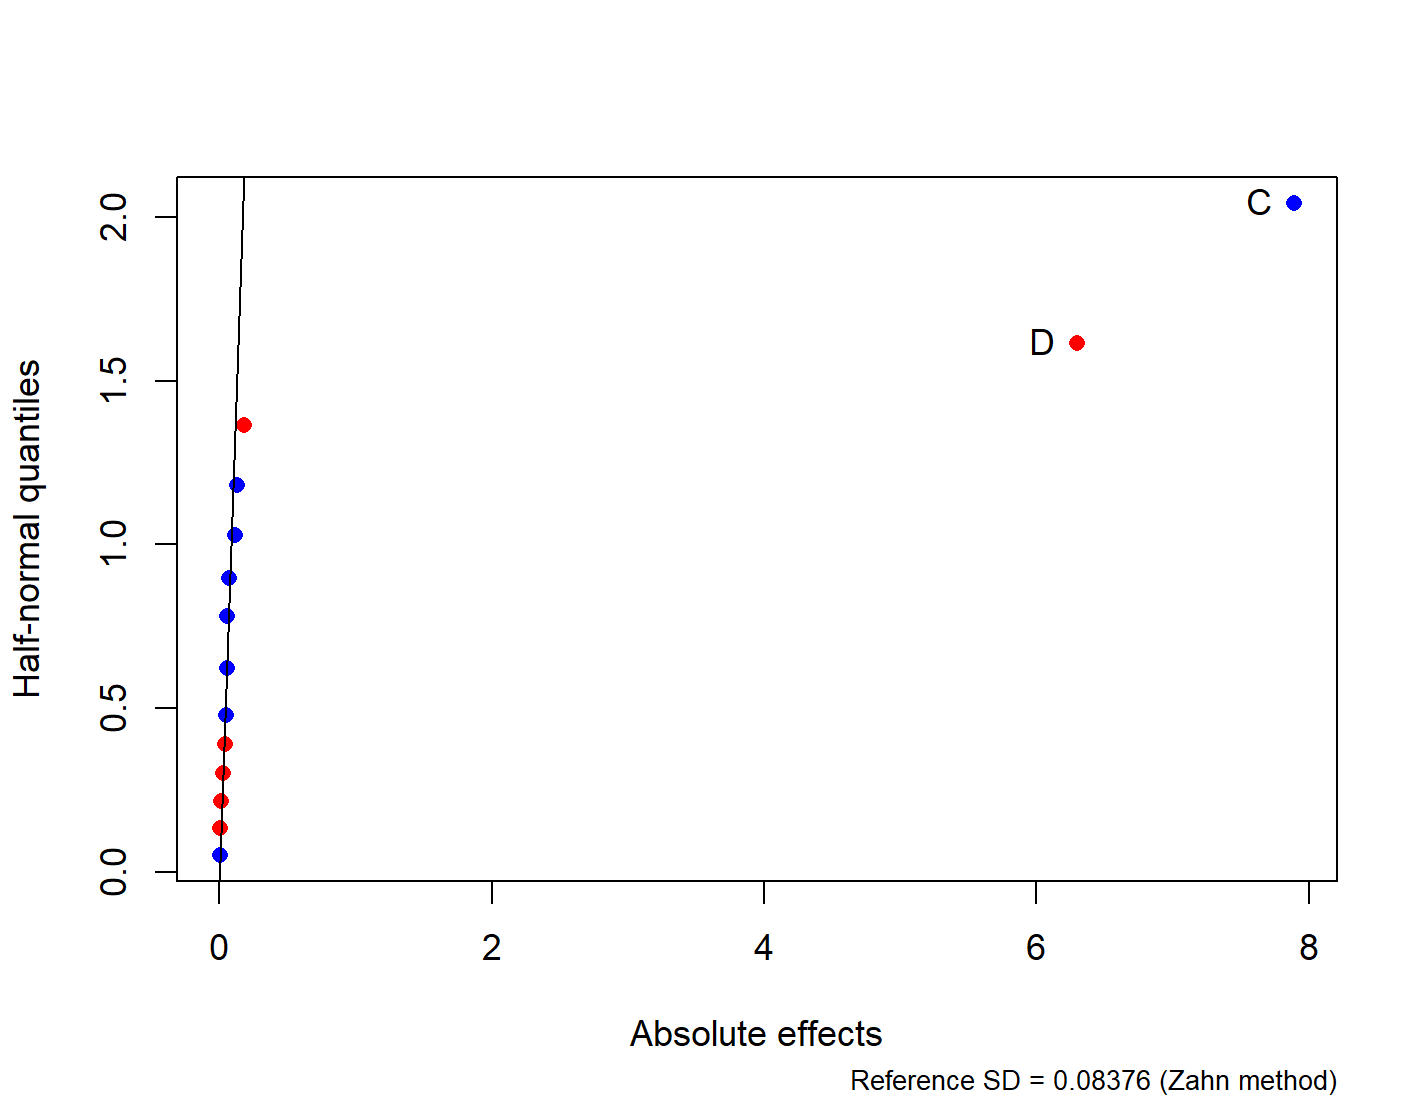
\includegraphics[width=0.7\columnwidth]{../images/chap_results/halfnormal.png}
    \caption[Phase I half-normal effects plot]{Half-normal probability plot of the Phase I effect estimates from Yates's algorithm. Effects that deviate substantially from the reference line are considered active \cite{montgomery2017design}. Only active effects are labeled.}
    \label{fig:results-p1-halfnormal}
\end{figure}

Factor C (APViT guidance) produced the largest main effect at +7.889 percentage points (pp), followed by factor D (dataset) at -6.297 pp, indicating that the AffectNet-7 subset yields higher accuracy than AffectNet-8. Factors A (pretrained backbone weights) and B (local-global feature extraction modules) showed negligible effects of +0.129 pp and +0.056 pp, respectively. All interaction effects were also negligible: the C×D interaction was +0.025 pp, and all remaining two-factor and higher-order interactions fell below 0.18 pp in absolute value. The within-cell standard deviations, obtained after pooling A and B, ranged from 0.08\% to 0.25\%, confirming that A and B contribute no meaningful variance to the response.\\

The C×D interaction quantifies whether the benefit of APViT guidance varies across datasets. The near-zero interaction estimate of +0.025 pp indicates that the contributions of C and D are negligible. Figure \ref{fig:results-p1-interaction} shows the interaction line plot for C and D after pooling A and B.\\

\begin{figure}[h!]
    \centering
    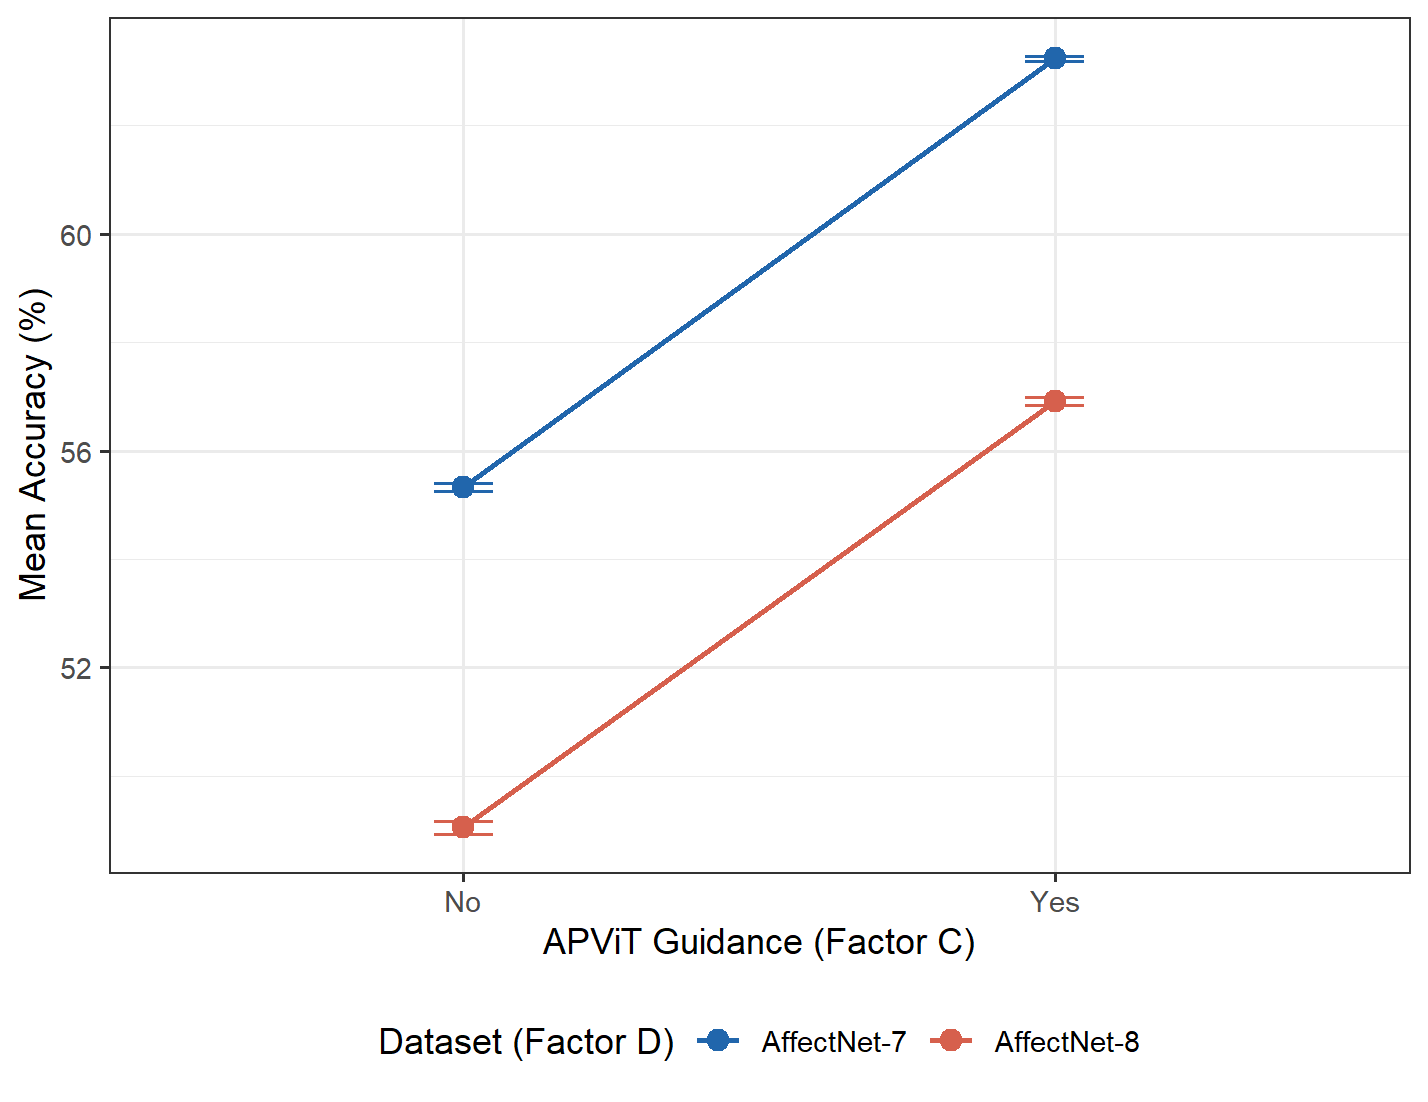
\includegraphics[width=0.7\columnwidth]{../images/chap_results/cxd_interaction.png}
    \caption[Phase I C×D interaction plot]{Interaction plot for factors C (APViT guidance) and D (dataset) after pooling negligible factors A and B. The near-parallel lines confirm the negligible C×D interaction (+0.025 pp).}
    \label{fig:results-p1-interaction}
\end{figure}

\subsection{Learning behavior}
\label{section:results-phase1-curves}

Training and validation accuracy curves were recorded for all 16 Phase I runs via WandB. Figure \ref{fig:results-p1-curves} presents representative curves for the four C×D conditions.\\

\begin{figure}[h!]
    \centering
    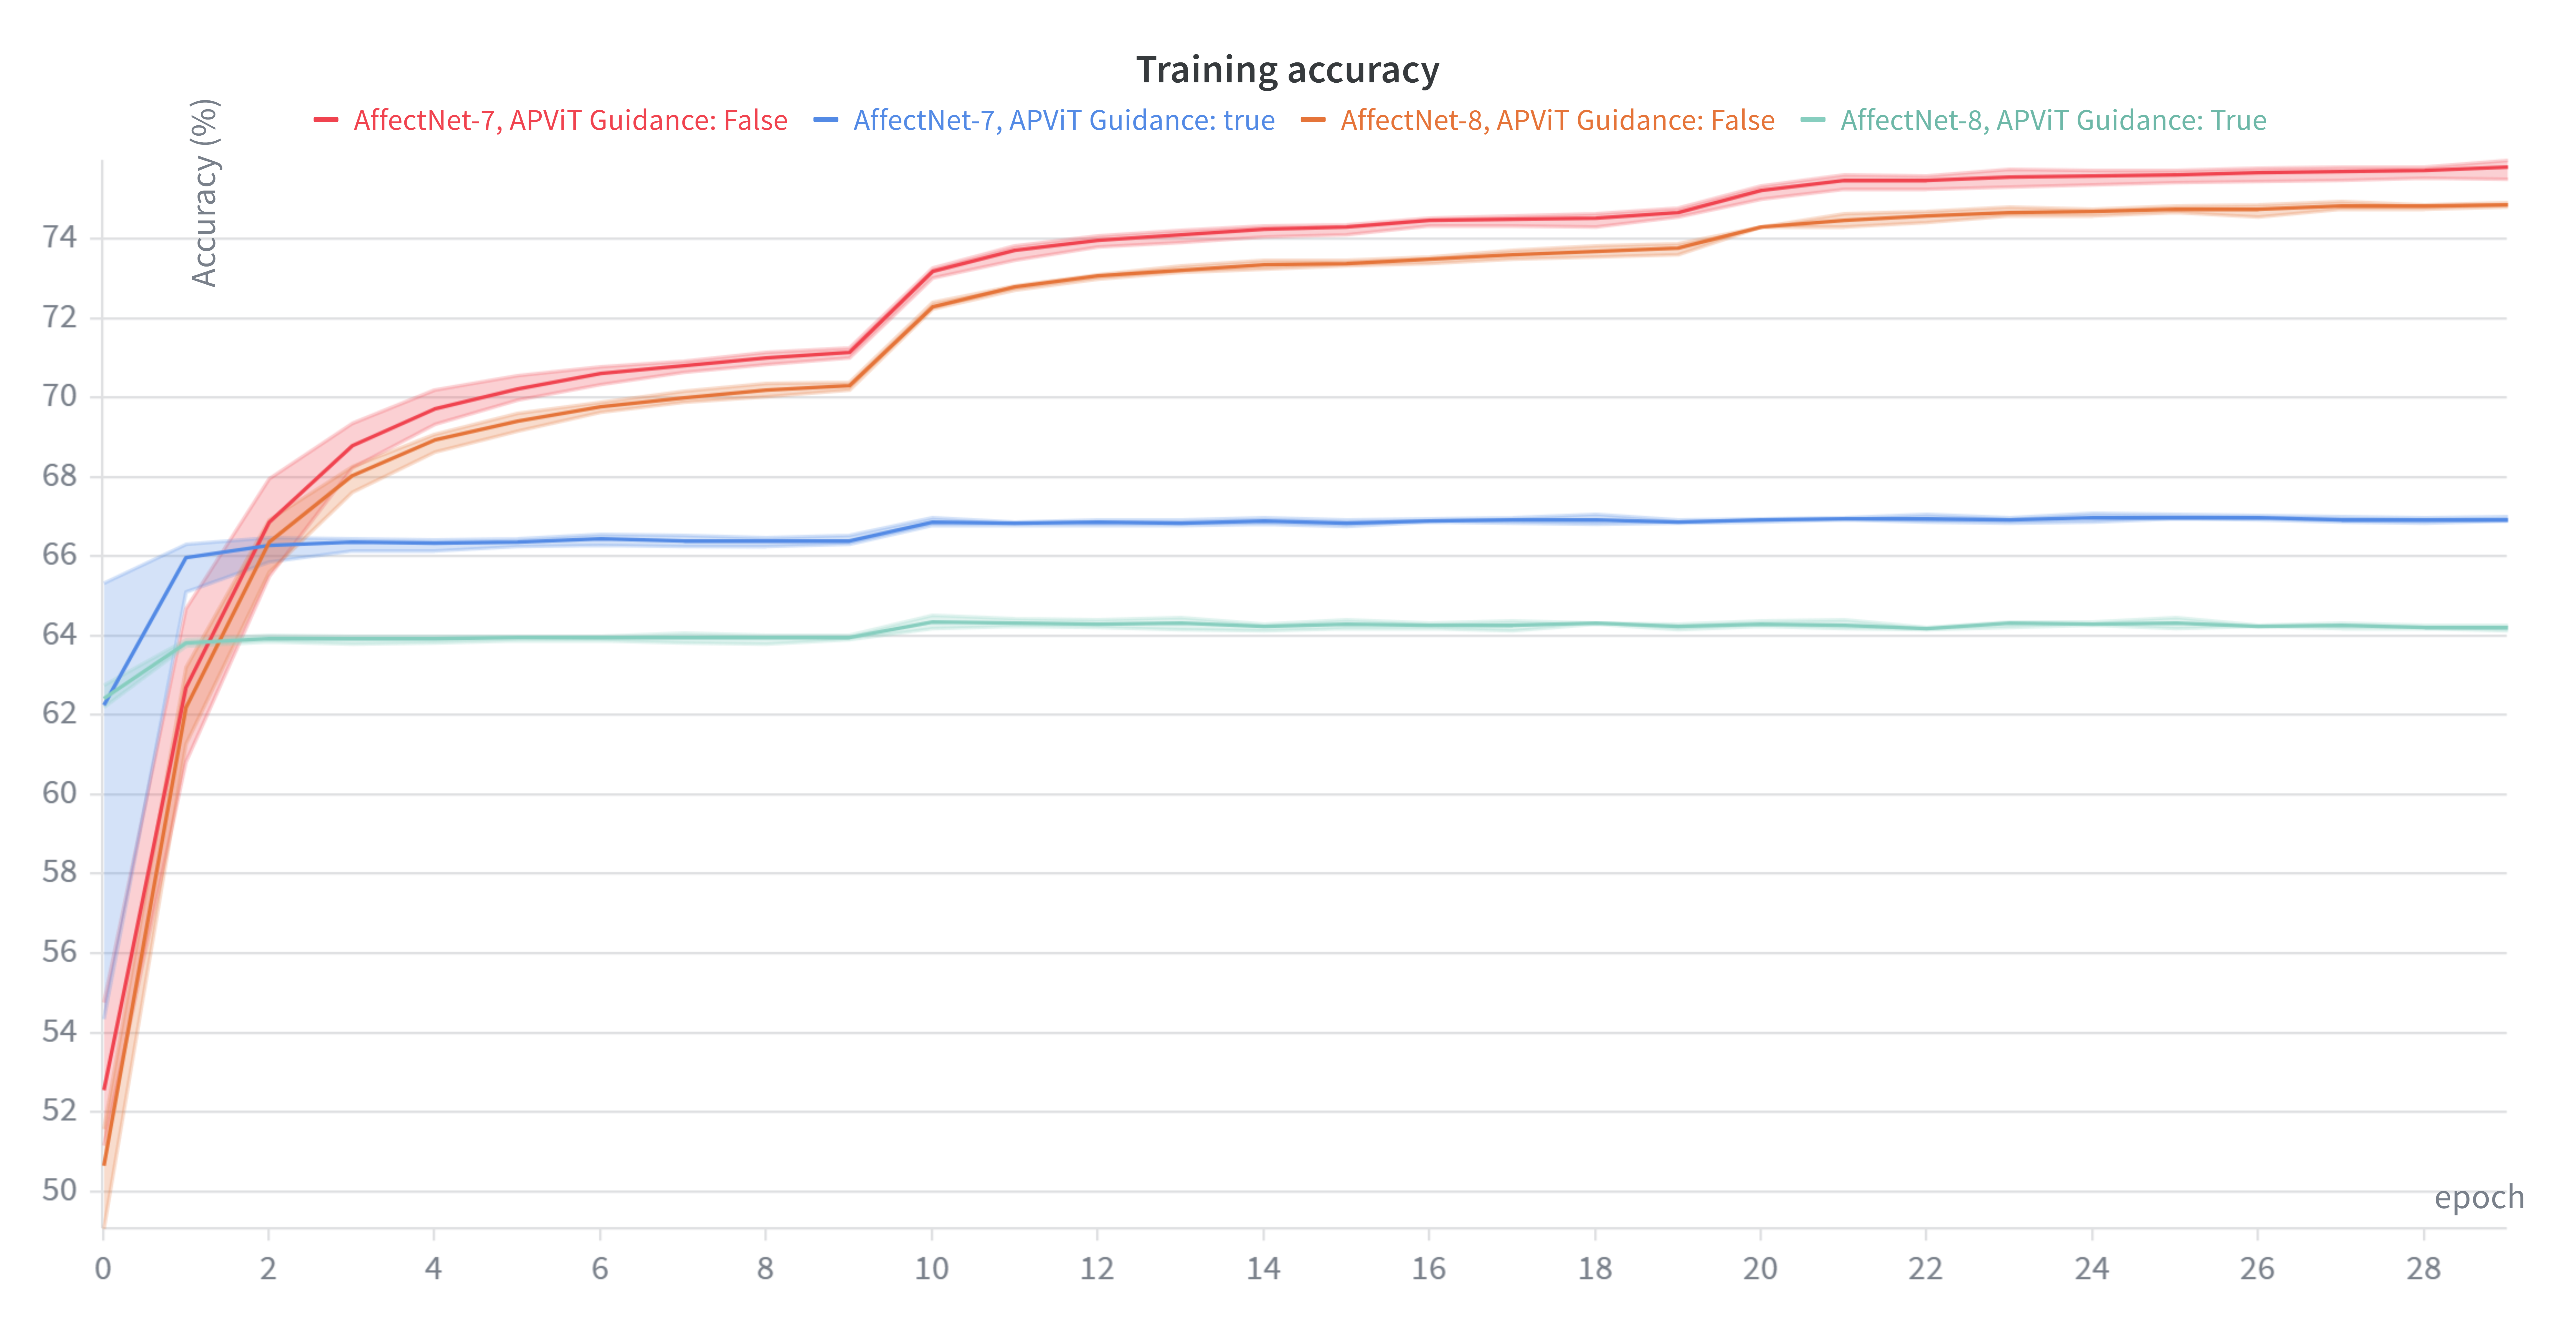
\includegraphics[width=1\columnwidth]{../images/chap_results/trainingcurve.png}
    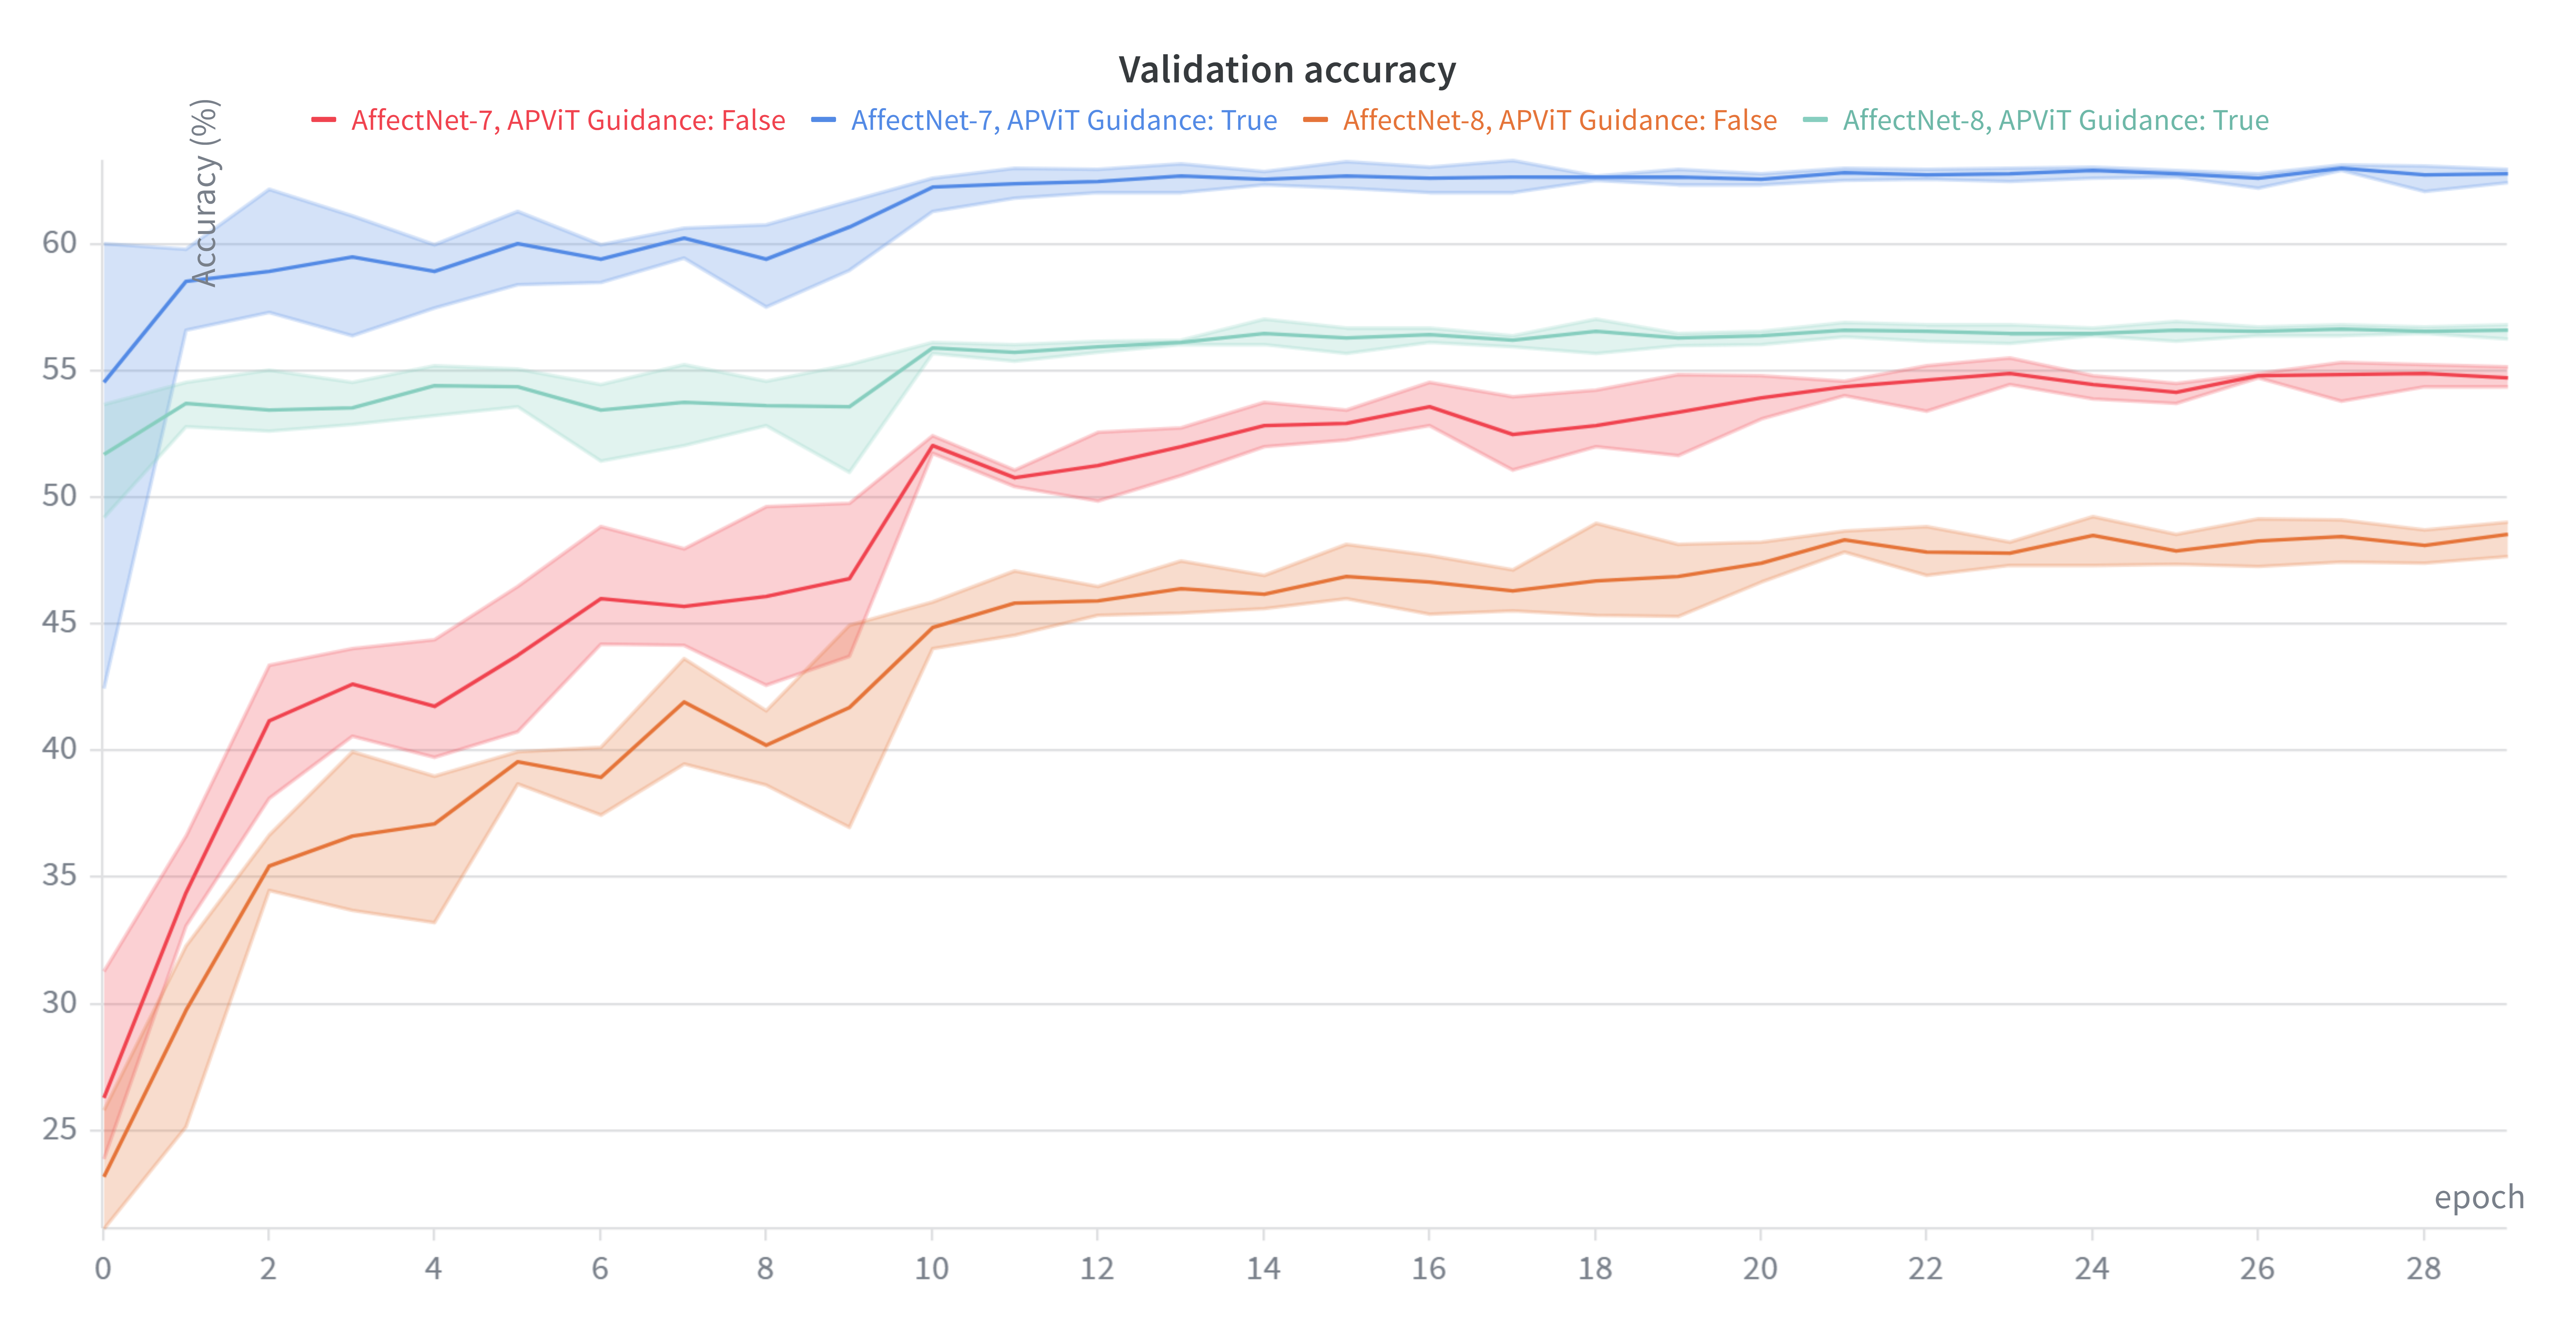
\includegraphics[width=1\columnwidth]{../images/chap_results/validationcurve.png}
    \caption[Phase I training curves by C×D condition]{Representative training and validation accuracy curves for the four C×D conditions in Phase I. Each curve aggregates runs (mean) within the same C×D cell across varying A and B levels.}
    \label{fig:results-p1-curves}
\end{figure}

We observe two distinct training behaviors depending on the state of factor C. Runs with APViT guidance (C+) converged to their best validation accuracy between epochs 13 and 27, with a mean train-validation gap of approximately 5-7\%. Runs without APViT guidance (C-) exhibited severe overfitting, with training accuracy reaching 75-76\% while validation accuracy plateaued early, yielding a mean train-validation gap of approximately 24\%. The learning rate schedule, which applies a decay factor at epochs 10 and 20, produced visible accuracy steps in C- runs that are attenuated or absent in C+ runs. Across all conditions, runs trained on AffectNet-8 plateaued approximately 6 pp below their AffectNet-7 counterparts.\\

\subsection{Hyperparameter optimization and the M-LDG}
\label{section:results-phase1-optim}

Following the factorial experiment, a Bayesian hyperparameter search using WandB Sweeps with Hyperband early termination \cite{hyperband2018} was applied to the two best-performing factor combinations for each dataset (0, 1, 5, and 12). Eight 12-epoch trials were conducted across the two datasets, after which the best-identified configurations were confirmed with full 30-epoch runs. Table \ref{tab:results-p1-sweep} reports all eight sweep trials.\\

\begin{table}[h!]
    \centering
    \begin{tabular}{@{}rllllllr@{}}
    \toprule
    \textbf{\#} & \textbf{Dataset} & \textbf{LR} & \textbf{M} & \textbf{WD} & \textbf{F} & \textbf{Freq.} & \textbf{Best Acc.\ (\%)} \\
    \midrule
    1 & AN-7 & 0.00205 & 0.865 & $5.08\times10^{-3}$ & 0.561 & 12 & \textbf{64.77} \\
    2 & AN-7 & 0.00205 & 0.944 & $1.35\times10^{-6}$ & 0.193 & 10 & 63.97 \\
    3 & AN-7 & 0.01461 & 0.861 & $2.50\times10^{-6}$ & 0.138 & 10 & 63.89 \\
    4 & AN-7 & 0.04980 & 0.888 & $8.01\times10^{-6}$ & 0.338 &  5 & 63.46 \\
    5 & AN-7 & 0.02782 & 0.931 & $1.76\times10^{-5}$ & 0.600 &  8 & 63.20 \\
    \midrule
    6 & AN-8 & 0.01856 & 0.932 & $1.16\times10^{-6}$ & 0.474 &  3 & \textbf{57.49} \\
    7 & AN-8 & 0.02003 & 0.937 & $1.37\times10^{-6}$ & 0.516 &  3 & 57.29 \\
    8 & AN-8 & 0.00430 & 0.885 & $4.09\times10^{-6}$ & 0.543 & 12 & 57.21 \\
    \bottomrule
    \end{tabular}
    \caption[Phase I hyperparameter sweep results]{Hyperparameter configurations and best validation accuracies for the eight Phase I sweep trials. Accuracy values are from 12-epoch runs with Hyperband early termination. M = Momentum, WD = Weight Decay, F = Factor, Freq = Frequency.}
    \label{tab:results-p1-sweep}
\end{table}

The resulting optimized network, achieved 64.34\% on AffectNet-7 (best epoch: 9) and 57.71\% on AffectNet-8 (best epoch: 12) in their respective 30-epoch confirmatory runs. These results represent improvements of +1.03 pp and +0.65 pp over the best ablation runs with C=True (63.31\% and 57.06\%). This optimized variant is used as the singular M-LDG network in the next phase of this study. Table \ref{tab:results-p1-hyperparams} compares the default and optimized hyperparameter configurations used to train the M-LDG.\\

\begin{table}[h!]
    \centering
    \begin{tabular}{@{}lllll@{}}
    \toprule
    \textbf{Parameter} & \shortstack{\textbf{Default}\\\textbf{(Ablation)}} & \shortstack{\textbf{Optimized}\\\textbf{(AN-7)}} & \shortstack{\textbf{Optimized}\\\textbf{(AN-8)}} & \textbf{Change} \\
    \midrule
    Learning Rate  & 0.100                       & 0.024                     & 0.032                     & $\downarrow$ 3--4$\times$ lower \\
    Momentum       & 0.900                       & 0.860                     & 0.948                     & Dataset-specific \\
    Weight Decay   & $1.0\times10^{-4}$          & $8.8\times10^{-6}$        & $1.5\times10^{-6}$        & $\downarrow$ 10--70$\times$ lower \\
    LR Factor      & 0.100                       & 0.209                     & 0.450                     & $\uparrow$ Less aggressive \\
    Adjust Freq    & 10                          & 10                        & 3                         & Dataset-specific \\
    \bottomrule
    \end{tabular}
    \caption[Phase I default vs. optimized hyperparameters]{Default (ablation) and optimized hyperparameter configurations for the M-LDG on each AffectNet subset. Arrows indicate the direction of change relative to the default.}
    \label{tab:results-p1-hyperparams}
\end{table}

The optimized configurations differ from the defaults in three main respects: the learning rate is 3 to 4 times lower, the weight decay is 10 to 70 times lower, and the LR reduction factor is substantially less aggressive (0.209 for AffectNet-7 and 0.450 for AffectNet-8, compared to the default of 0.1). The AffectNet-7 M-LDG converged rapidly, reaching within 0.5 pp of its best accuracy by epoch 6, with a final train-validation gap of 2.71 pp. The AffectNet-8 M-LDG required more epochs to stabilize, with a final gap of 7.19 pp, reflecting the increased difficulty of the 8-class task.\\

\section{Statistical assumption tests}
\label{section:results-assumptions}

Prior to the two-way ANOVA, we verified the normality of residuals and the homogeneity of variance as required by the ANOVA assumptions. Both assumption tests were conducted on the Phase I data after pooling the negligible factors A and B into the error term, retaining C and D as the active factors.\\

The Shapiro-Wilk test for normality of residuals yielded $W = 0.9447$ ($p = 0.410$), providing no evidence against the normality assumption. Levene's test for homogeneity of variance produced $F(3, 12) = 1.317$ ($p = 0.314$), indicating no significant difference in variance across the four C×D cells. Both assumptions for parametric ANOVA are therefore satisfied. Figure \ref{fig:results-assumptions} shows the normal Q-Q plot of residuals and the residuals-versus-fitted plot used to assess these assumptions visually.\\

\begin{figure}[h!]
    \centering
    \begin{minipage}{0.49\columnwidth}
        \centering
        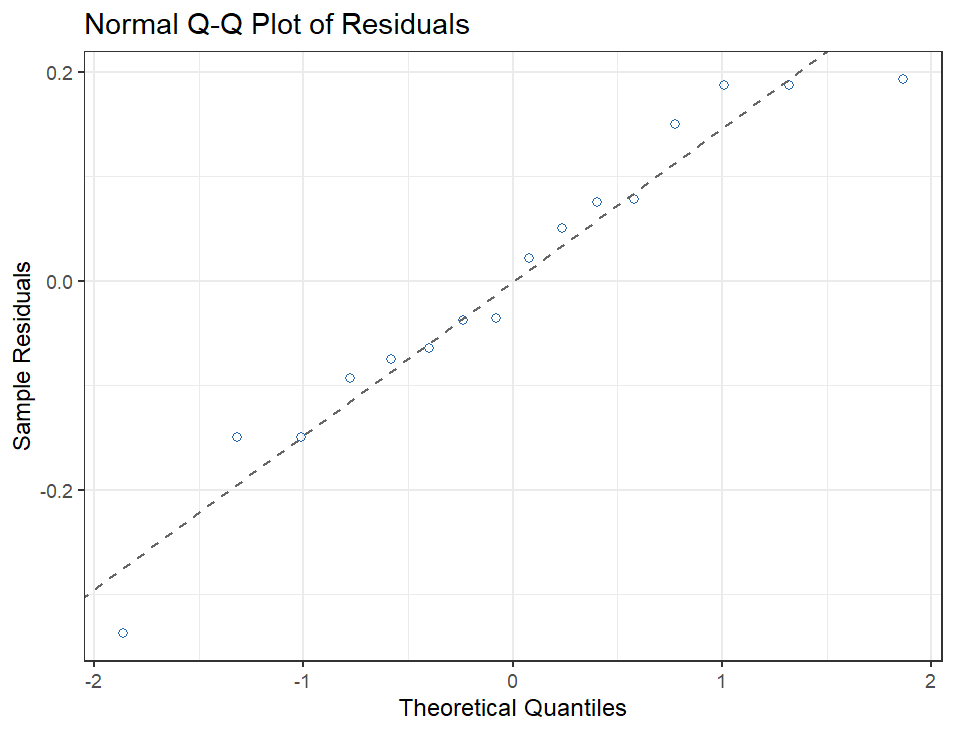
\includegraphics[width=\linewidth]{../images/chap_results/normalqq.png}
    \end{minipage}\hfill
    \begin{minipage}{0.49\columnwidth}
        \centering
        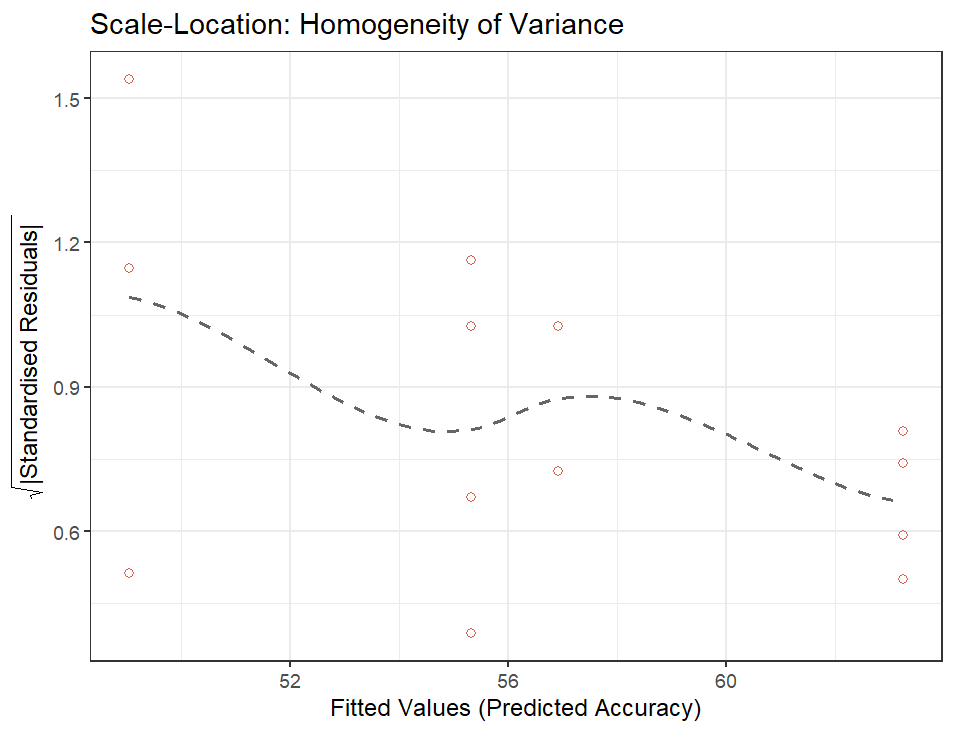
\includegraphics[width=\linewidth]{../images/chap_results/homovar.png}
    \end{minipage}
    \caption[Phase I ANOVA assumption plots]{Phase I ANOVA assumption checks after pooling factors A and B. Left: normal Q-Q plot of residuals; close alignment with the reference diagonal supports normality (Shapiro-Wilk $W = 0.9447$, $p = 0.410$). Right: residuals versus fitted values for the two-way ANOVA model; relatively constant spread suggests homoscedasticity, confirmed by Levene's test ($F(3, 12) = 1.317$, $p = 0.314$).}
    \label{fig:results-assumptions}
\end{figure}

\section{Two-way ANOVA results}
\label{section:results-anova}

A two-way ANOVA was performed on the Phase I data with best validation accuracy as the response and APViT guidance (C) and dataset (D) as the predictors, following the procedure defined in the \nameref{chapter:methodology} chapter. Given their low effect estimates, we pool together factors A and B to increase the reliability of the results. The criteria for pooling is based on visual analysis via the half-normal plot in Figure \ref{fig:results-p1-halfnormal}. Table \ref{tab:results-anova} presents the ANOVA table.\\

\begin{table}[h!]
    \centering
    \begin{tabular}{@{}lrrrrl@{}}
    \toprule
    \textbf{Source} & \textbf{df} & \textbf{SS} & \textbf{MS} & \textbf{F} & \textbf{$p$-value} \\
    \midrule
    APViT guidance (C)  & 1  & 248.97 & 248.97 & 9196.84 & $< 2\times10^{-16}$\,*** \\
    Dataset (D)         & 1  & 158.59 & 158.59 & 5858.17 & $< 2\times10^{-16}$\,*** \\
    C $\times$ D        & 1  &   0.002 &   0.002 &   0.092 & 0.767\phantom{$\times10^{-16}$\,***} \\
    Residuals           & 12 &   0.325 &   0.027 & & \\
    \bottomrule
    \end{tabular}
    \smallskip

    \footnotesize{Significance codes: *** $p < 0.001$. Factors A and B were pooled into the residuals.}
    \caption[Phase I two-way ANOVA]{Two-way ANOVA results for Phase I. Factors A and B were pooled into the residual after the effect estimation step; the model retains only factors C (APViT guidance) and D (dataset).}
    \label{tab:results-anova}
\end{table}

Both main effects were highly significant, while their interaction was not. APViT guidance (C) yielded $F(1, 12) = 9196.84$ ($p < 2 \times 10^{-16}$), the dataset (D) yielded $F(1, 12) = 5858.17$ ($p < 2 \times 10^{-16}$), and the C×D interaction was negligible ($F(1, 12) = 0.092$, $p = 0.767$). The residual term in Table \ref{tab:results-anova} is very small: repeated runs under the same condition landed within roughly 0.16 percentage points of one another, so the observed differences between conditions are highly reproducible rather than the product of random fluctuation.\\

To measure how much each factor matters in practice, we report effect sizes as eta-squared ($\eta^2$), the proportion of the total variation in accuracy explained by a factor. Dividing each factor's sum of squares in Table \ref{tab:results-anova} by the total sum of squares (407.89) gives $\eta^2 = 0.610$ for APViT guidance and $\eta^2 = 0.389$ for the dataset, with the interaction below 0.001. Together these two factors explain about 99.9\% of the systematic variation in accuracy. We therefore reject the null hypothesis that all treatment combinations yield the same mean accuracy: both APViT guidance and the choice of dataset produce statistically significant differences in performance.\\

\section{Phase II: EfficientFace guidance comparison}
\label{section:results-phase2}

\subsection{Cell means and replication}
\label{section:results-phase2-cells}

Phase II employed a $2^2$ factorial design with two replicates per treatment combination, as described in Table~\ref{tab:p2-runs}. The two factors were guidance network (G: M-LDG or APViT) and dataset (D: AffectNet-7 or AffectNet-8). A total of eight EfficientFace training runs were conducted, each for 45 epochs. Table \ref{tab:results-p2-cells} reports the individual run results and cell means.\\

\begin{table}[h!]
    \centering
    \begin{tabular}{@{}llrrrrl@{}}
    \toprule
    \textbf{Guidance (G)} & \textbf{Dataset (D)} & \textbf{Rep.\ 1} & \textbf{Rep.\ 2} & \textbf{Cell Mean} & \textbf{SD} & \textbf{$n$} \\
    \midrule
    APViT  & AffectNet-7 & 62.31 & 61.89 & 62.10 & 0.303 & 2 \\
    APViT  & AffectNet-8 & 56.11 & 55.49 & 55.80 & 0.442 & 2 \\
    M-LDG  & AffectNet-7 & 63.00 & 62.43 & 62.71 & 0.404 & 2 \\
    M-LDG  & AffectNet-8 & 55.99 & 55.81 & 55.90 & 0.124 & 2 \\
    \bottomrule
    \end{tabular}
    \caption[Phase II cell means and replicate results]{Phase II best validation accuracy (\%) for each run, cell means, and within-cell standard deviations. Each cell contains two replicates of EfficientFace trained with the specified guidance network on the specified dataset.}
    \label{tab:results-p2-cells}
\end{table}

The M-LDG-guided conditions achieved cell means of 62.71\% on AffectNet-7 (SD = 0.404\%) and 55.90\% on AffectNet-8 (SD = 0.124\%). The APViT-guided conditions achieved 62.10\% (SD = 0.303\%) and 55.80\% (SD = 0.442\%), respectively. 
%The $2^2$ factorial effects were estimated by ordinary least squares (\texttt{lm(best\_accuracy \textasciitilde{} G * D)}) using $\pm1$ contrast coding (G: APViT $=-1$, M-LDG $=+1$; D: AffectNet-7 $=-1$, AffectNet-8 $=+1$), so that each coefficient equals half the difference between the corresponding factor levels and the level contrast (high $-$ low) is twice the coefficient. The estimated grand mean was 59.129\%. The guidance-network coefficient was $+0.179$ pp (SE $=0.121$, $t(4) = 1.480$, $p = 0.213$), equivalent to a $+0.357$ pp contrast in favor of M-LDG. The dataset coefficient was $-3.278$ pp (SE $=0.121$, $t(4) = -27.167$, $p = 1.09\times10^{-5}$), equivalent to a $-6.556$ pp contrast that is consistent with the dataset effect observed in Phase I. The G$\times$D interaction coefficient was $-0.129$ pp (SE $=0.121$, $t(4) = -1.066$, $p = 0.347$); its negative sign indicates that the M-LDG advantage was +0.614 pp on AffectNet-7 but only +0.100 pp on AffectNet-8. The model accounted for almost all between-cell variance ($R^2 = 0.995$, adjusted $R^2 = 0.991$; $F(3,4) = 247.1$, $p = 5.39\times10^{-5}$), but only the dataset factor reached statistical significance. 
Figure \ref{fig:results-p2-bars} shows the cell means with error bars.

\begin{figure}[h!]
    \centering
    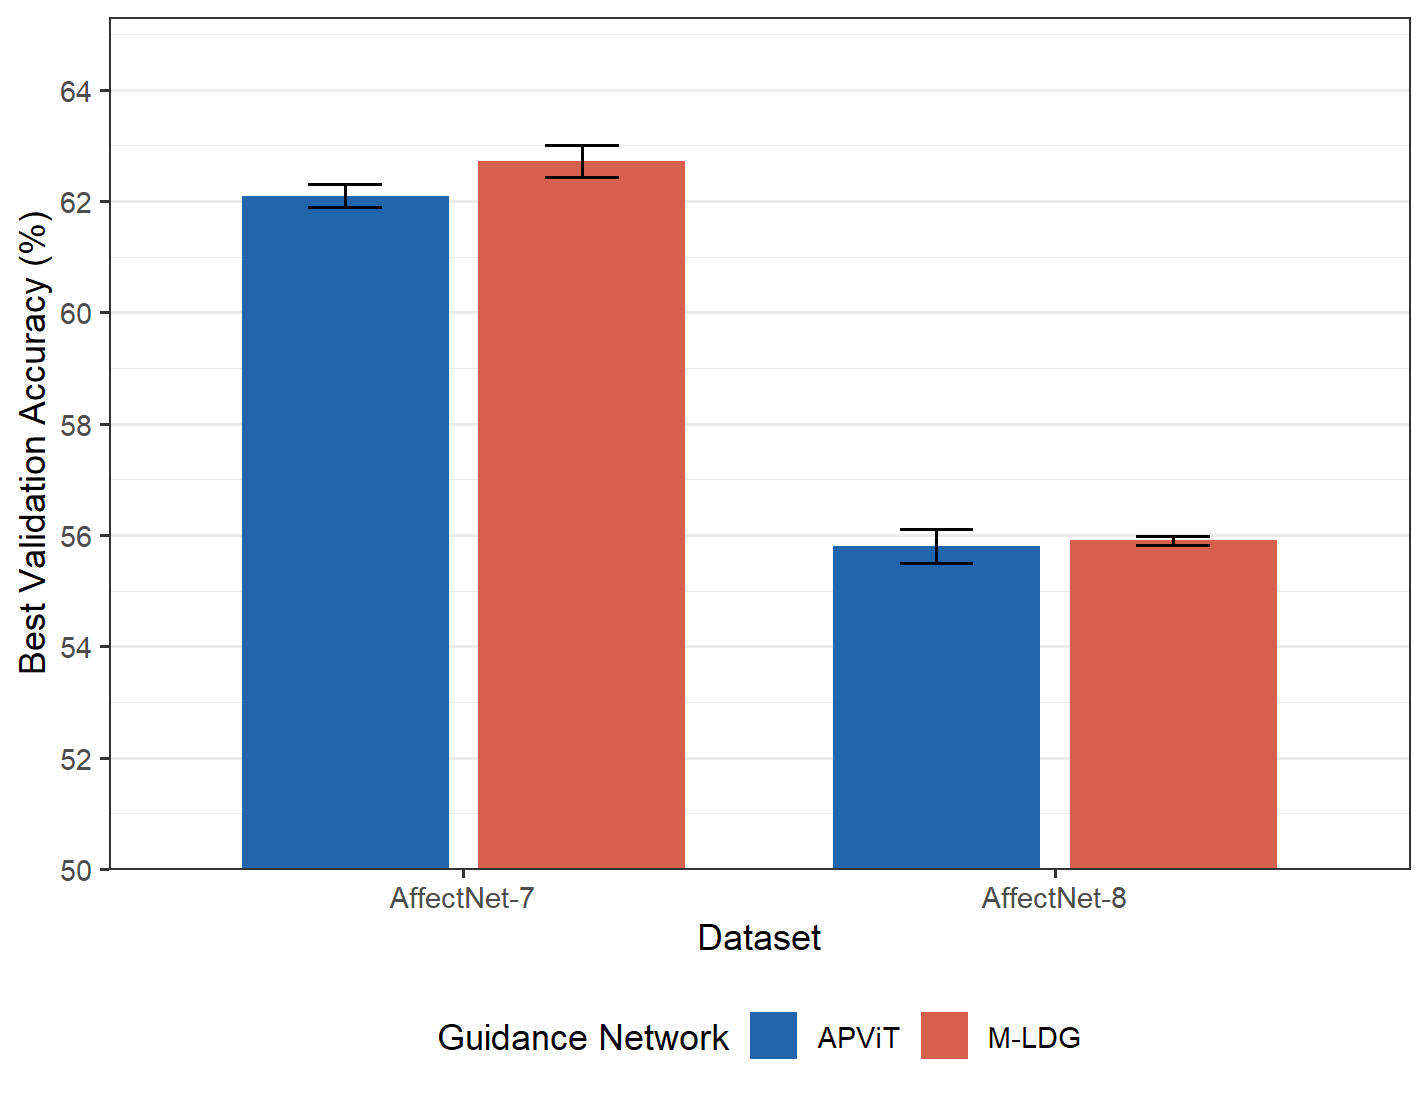
\includegraphics[width=1\columnwidth]{../images/chap_results/phase2comp.png}
    \caption[Phase II cell means bar chart]{Cell means for EfficientFace best validation accuracy under each guidance network and dataset condition in Phase II. Error bars indicate the range between the two replicates in each cell.}
    \label{fig:results-p2-bars}
\end{figure}

\subsection{Significance testing}
\label{section:results-phase2-significance}

Welch's t-tests were applied separately for each dataset to compare the mean accuracy of M-LDG-guided and APViT-guided EfficientFace, as specified in the \nameref{chapter:methodology} chapter.\\

For AffectNet-7, the mean accuracy was 62.71\% for M-LDG (SD = 0.404\%) and 62.10\% for APViT (SD = 0.303\%). The observed difference was +0.614 pp in favor of the M-LDG. The Welch t-test yielded $t(1.85) = -1.720$ with $p = 0.237$ and a 95\% confidence interval of $[-1.044,\ 2.272]$ pp. For AffectNet-8, the mean accuracy was 55.90\% for M-LDG (SD = 0.124\%) and 55.80\% for APViT (SD = 0.442\%). The observed difference was +0.100 pp in favor of the M-LDG. The Welch t-test yielded $t(1.16) = -0.308$ with $p = 0.804$ and a 95\% confidence interval of $[-2.917,\ 3.117]$ pp.\\

Neither comparison reached statistical significance. The wide confidence intervals spanning zero in both cases indicate that the direction of the difference cannot be established at the current sample size. With $n = 2$ replicates per cell, the Phase II tests are severely underpowered and can only detect very large effects; the failure to reach significance should be interpreted as inconclusive rather than as evidence of equivalence between M-LDG and APViT as guidance networks for EfficientFace.\\

\subsection{Hyperparameter optimization}
\label{section:results-phase2-optim}

Following the same Bayesian sweep procedure as Phase I, hyperparameter optimization was applied to two Phase II conditions: M-LDG with AffectNet-7 and APViT with AffectNet-8. Five 20-epoch sweep trials were conducted per combination, followed by 65-epoch confirmatory runs using the best identified configuration.\\

The optimized confirmatory runs achieved 62.29\% for M-LDG on AffectNet-7 and 55.01\% for APViT on AffectNet-8. These are lower than the corresponding Phase II baseline runs conducted with default hyperparameters, which achieved 63.00\% and 56.11\%, respectively. The differences represent decreases of -0.43 pp and -0.45 pp. Hyperparameter optimization in Phase II therefore produced a negative result: the default training configuration (learning rate 0.1, momentum 0.9, weight decay $10^{-4}$, LR factor 0.1, adjustment frequency 10) outperformed all optimized configurations identified by the sweep.\\

\section{Additional obtained metrics}
\label{section:results-metrics}

\subsection{Cross-phase accuracy progression}
\label{section:results-metrics-progression}

To summarize the accuracy gains at each stage of the proposed pipeline, Table \ref{tab:results-progression} presents the cross-phase accuracy progression from the unguided LDG baseline through to the final EfficientFace variants. This table directly addresses specific objective 3 from the \nameref{chapter:hypothesis-objectives} chapter, which calls for training two EfficientFace variants and studying their performance relative to the baseline and to each other.\\

\begin{table}[h!]
    \centering
    \begin{tabular}{@{}lrr@{}}
    \toprule
    \textbf{Stage} & \textbf{AffectNet-7} & \textbf{AffectNet-8} \\
    \midrule
    M-LDG baseline (C=False, ablation)             & 55.51 & 49.24 \\
    M-LDG + APViT guidance (C=True, ablation)      & 63.31 & 57.06 \\
    M-LDG (Phase I optimized)                    & \textbf{64.34} & \textbf{57.71} \\
    EfficientFace guided by M-LDG (Phase II)     & 63.00 & 55.99 \\
    EfficientFace guided by APViT (Phase II)     & 62.31 & 56.11 \\
    \midrule
    Published EfficientFace \cite{eff-face2021} & 63.70 & 59.89 \\
    Published APViT \cite{apvit2023}            & 66.91 & --- \\
    APViT trained from scratch                  & 64.2 & 57.31 \\
    \bottomrule
    \end{tabular}
    \caption[Cross-phase accuracy progression]{Accuracy (\%) at each stage of the proposed knowledge transfer pipeline for both AffectNet subsets. Published baselines from \cite{eff-face2021} and \cite{apvit2023} are provided for reference. We also present the performance of our own APViT model trained from scratch on AffectNet 7 and 8.}
    \label{tab:results-progression}
\end{table}

The unguided M-LDG baseline (C=False) achieved 55.51\% on AffectNet-7 and 49.24\% on AffectNet-8. Adding APViT knowledge distillation (C=True) raised accuracy to 63.31\% and 57.06\%, respectively. The M-LDG, after hyperparameter optimization, reached 64.34\% (AffectNet-7) and 57.71\% (AffectNet-8). EfficientFace trained with M-LDG-generated soft labels achieved 63.00\% (AffectNet-7) and 55.99\% (AffectNet-8), while EfficientFace trained with APViT-generated soft labels achieved 62.31\% and 56.11\%. For reference, the original EfficientFace authors report 63.7\% on AffectNet \cite{eff-face2021} and the APViT teacher used in this study reports 66.91\% on AffectNet \cite{apvit2023}.\\

\subsection{Per-class behavior}
\label{section:results-metrics-perclass}

In addition to the top-1 accuracy response variable, per-class validation confusion matrices were logged for all runs via WandB. We report here the confusion matrices for the best M-LDG-guided EfficientFace variants obtained in Phase II: the AffectNet-7 model (63\% best accuracy) and the AffectNet-8 model (55.99\% best accuracy). These matrices capture the distribution of correct and incorrect predictions across expression classes and complement the main accuracy reported throughout this chapter.\\

Figure \ref{fig:results-cm-an7} shows the normalized confusion matrix for the best M-LDG-guided EfficientFace on AffectNet-7 and figure \ref{fig:results-cm-an8} shows the corresponding matrix for AffectNet-8.\\

\begin{figure}[h!]
    \centering
    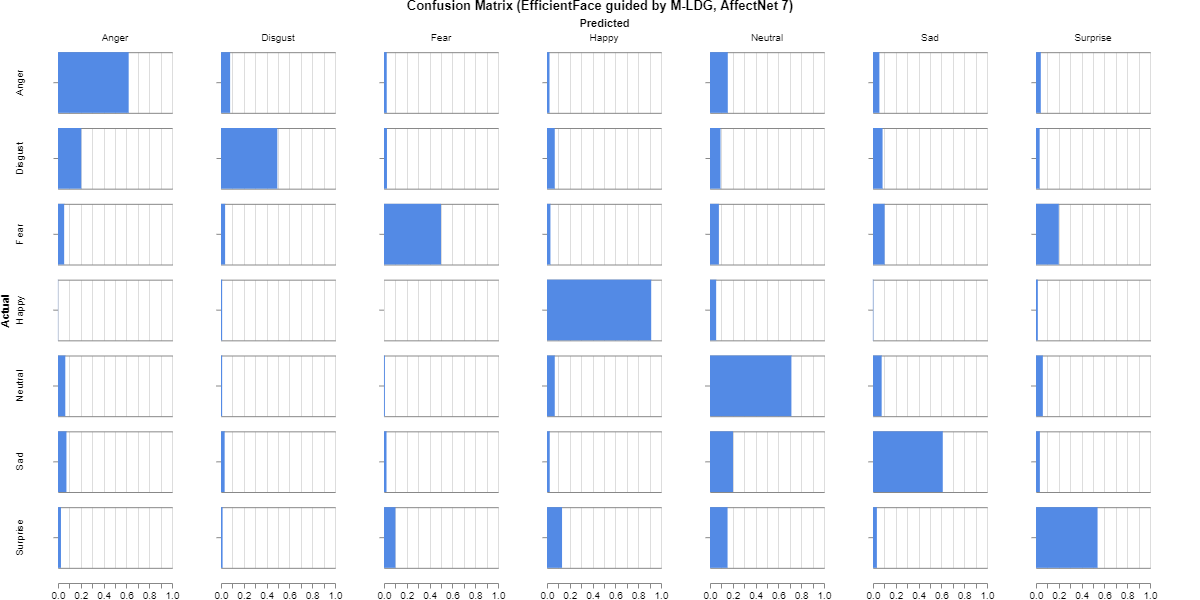
\includegraphics[width=1\columnwidth]{../images/chap_results/7classconf.png}
    \caption[Confusion matrix: M-LDG EfficientFace on AffectNet-7]{Normalized confusion matrix for the best M-LDG-guided EfficientFace variant on AffectNet-7. Rows represent true classes; columns represent predicted classes. Values indicate the fraction of samples in each true-class row assigned to each predicted class.}
    \label{fig:results-cm-an7}
\end{figure}

\begin{figure}[h!]
    \centering
    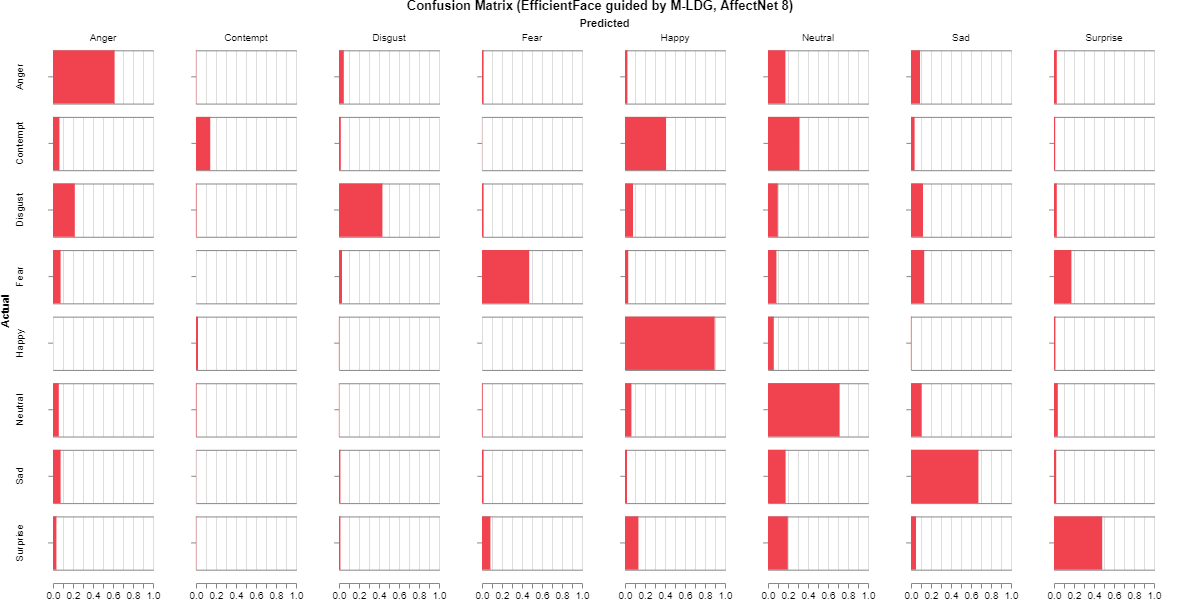
\includegraphics[width=1\columnwidth]{../images/chap_results/8classconf.png}
    \caption[Confusion matrix: M-LDG EfficientFace on AffectNet-8]{Normalized confusion matrix for the best M-LDG-guided EfficientFace variant on AffectNet-8, including the contempt class. Rows and columns follow the same convention as figure \ref{fig:results-cm-an7}.}
    \label{fig:results-cm-an8}
\end{figure}

\subsection{Per-class and macro-averaged metrics}
\label{section:results-metrics-classmetrics}

Beyond the top-1 accuracy response variable, we computed per-class and macro-averaged classification metrics for the five pipeline stages of table \ref{tab:results-progression} on both AffectNet subsets, derived from the same logged confusion matrices used in section \ref{section:results-metrics-perclass}. These metrics were not subjected to the formal statistical analysis applied to top-1 accuracy in Phases I and II and are reported here as descriptive summaries only. Table \ref{tab:results-perclass-acc} reports per-class recall, and table \ref{tab:results-macro} reports the macro-averaged precision, recall, and F1 score alongside top-1 accuracy for all ten trained models.\\

\begin{table}[h!]
    \centering
    \footnotesize
    \resizebox{\linewidth}{!}{%
    \begin{tabular}{@{}lrrrrr@{}}
    \toprule
    \multicolumn{6}{c}{\textbf{AffectNet-7}} \\
    \cmidrule(lr){2-6}
    \textbf{Emotion} & \textbf{M-LDG base} & \textbf{M-LDG+APViT} & \textbf{M-LDG optim.} & \textbf{EF+APViT} & \textbf{EF+M-LDG} \\
    \midrule
    Anger    & 0.562 & \textbf{0.660} & 0.654 & 0.656 & 0.622 \\
    Disgust  & 0.282 & 0.450 & \textbf{0.514} & 0.436 & 0.506 \\
    Fear     & 0.440 & \textbf{0.540} & 0.538 & 0.498 & 0.520 \\
    Happy    & \textbf{0.936} & 0.914 & 0.908 & 0.928 & 0.914 \\
    Neutral  & \textbf{0.784} & 0.726 & 0.716 & 0.700 & 0.704 \\
    Sad      & 0.518 & \textbf{0.642} & 0.634 & 0.622 & 0.618 \\
    Surprise & 0.364 & 0.500 & \textbf{0.540} & 0.522 & 0.526 \\
    \midrule
    \multicolumn{6}{c}{\textbf{AffectNet-8}} \\
    \cmidrule(lr){2-6}
    \textbf{Emotion} & \textbf{M-LDG base} & \textbf{M-LDG+APViT} & \textbf{M-LDG optim.} & \textbf{EF+APViT} & \textbf{EF+M-LDG} \\
    \midrule
    Anger    & 0.564 & 0.638 & \textbf{0.642} & \textbf{0.642} & 0.612 \\
    Contempt & 0.004 & 0.134 & \textbf{0.186} & 0.124 & 0.164 \\
    Disgust  & 0.286 & 0.460 & \textbf{0.466} & 0.450 & 0.452 \\
    Fear     & 0.444 & 0.504 & \textbf{0.522} & 0.502 & 0.478 \\
    Happy    & \textbf{0.950} & 0.920 & 0.894 & 0.908 & 0.898 \\
    Neutral  & \textbf{0.776} & 0.682 & 0.714 & 0.684 & 0.714 \\
    Sad      & 0.566 & \textbf{0.702} & 0.682 & 0.686 & 0.666 \\
    Surprise & 0.348 & \textbf{0.524} & 0.510 & 0.492 & 0.494 \\
    \bottomrule
    \end{tabular}%
    }
    \smallskip
    \caption[Per-class recall by pipeline stage]{Per-class recall for the five pipeline stages of table \ref{tab:results-progression} on both AffectNet subsets.}
    \label{tab:results-perclass-acc}
\end{table}

\begin{table}[h!]
    \centering
    \footnotesize
    \resizebox{\linewidth}{!}{%
    \begin{tabular}{@{}lrrrrr@{}}
    \toprule
    \multicolumn{6}{c}{\textbf{AffectNet-7}} \\
    \cmidrule(lr){2-6}
    \textbf{Metric} & \textbf{M-LDG base} & \textbf{M-LDG+APViT} & \textbf{M-LDG optim.} & \textbf{EF+APViT} & \textbf{EF+M-LDG} \\
    \midrule
    Top-1 Acc.\ (\%) & 55.51 & 63.31 & \textbf{64.34} & 62.31 & 63.00 \\
    Precision              & 0.626 & 0.653 & \textbf{0.658} & 0.647 & 0.643 \\
    Recall             & 0.555 & 0.633 & \textbf{0.643} & 0.623 & 0.630 \\
    F1                 & 0.543 & 0.629 & \textbf{0.641} & 0.618 & 0.627 \\
    \midrule
    \multicolumn{6}{c}{\textbf{AffectNet-8}} \\
    \cmidrule(lr){2-6}
    \textbf{Metric} & \textbf{M-LDG base} & \textbf{M-LDG+APViT} & \textbf{M-LDG optim.} & \textbf{EF+APViT} & \textbf{EF+M-LDG} \\
    \midrule
    Top-1 Acc.\ (\%) & 49.24 & 57.06 & \textbf{57.71} & 56.11 & 55.99 \\
    Precision              & \textbf{0.641} & 0.634 & 0.628 & 0.625 & 0.622 \\
    Recall             & 0.492 & 0.571 & \textbf{0.577} & 0.561 & 0.560 \\
    F1                 & 0.454 & 0.549 & \textbf{0.562} & 0.540 & 0.543 \\
    \bottomrule
    \end{tabular}%
    }
    \smallskip
    \caption[Macro-averaged validation metrics by pipeline stage]{Macro-averaged precision, recall, and F1 score with the corresponding top-1 validation accuracy (\%) for the five pipeline stages of table \ref{tab:results-progression} on both AffectNet subsets. Macro averages weight every class equally regardless of its sample count.}
    \label{tab:results-macro}
\end{table}

\subsection{Model complexity}
\label{section:results-metrics-complexity}

Table \ref{tab:results-complexity} reports the parameter and MFLOPs (floating-point operations) counts for the four architectures involved in the proposed pipeline alongside the best top-1 validation accuracy each achieved on AffectNet-7. Counts were computed using the \texttt{thop} library \cite{lyken17_thop}, with each multiply-accumulate (MAC) operation counted as one FLOP. The 7-class and 8-class variants of each model differ only in their final classification head, so the 7-class figures serve as representative values.\\

\begin{table}[h!]
    \centering
    \begin{tabular}{@{}lrrr@{}}
    \toprule
    \textbf{Model} & \textbf{Best Acc.\ (\%)} & \textbf{Params (M)} & \textbf{MFLOPs} \\
    \midrule
    M-LDG                                & 64.34 & 56.43 &  6334.4 \\
    EfficientFace (Phase II)                        & 63.00 &  1.28 &   158.6 \\
    Original LDG \cite{eff-face2021}   & ---   & 23.52 &  4131.7 \\
    APViT \cite{apvit2023}          & 66.91 & 65.06 & 12400.1 \\
    \bottomrule
    \end{tabular}
    \smallskip
    \caption[Model complexity summary]{Best AffectNet-7 accuracy, parameter count (in millions), and MFLOPs for the four architecture families under study. M-LDG variants share identical complexity, as do all EfficientFace variants. Original LDG accuracy on AffectNet is not reported in \cite{eff-face2021}.}
    \label{tab:results-complexity}
\end{table}

\subsection{Interpretability}
\label{section:results-metrics-cam}

To provide evidence of the spatial attention patterns learned by the main networks in our study, we apply class activation maps (CAMs) \cite{cams2016}. CAM visualizations highlight the image regions that contributed most strongly to the network's predicted class, offering a spatial perspective on model behavior that complements the quantitative accuracy metrics reported in the preceding sections.\\

Figure \ref{fig:results-cam} presents a grid of CAM visualizations for four of the five networks presented in the cross phase comparison (see table \ref{tab:results-progression}).\\

\begin{figure}[h!]
    \centering
    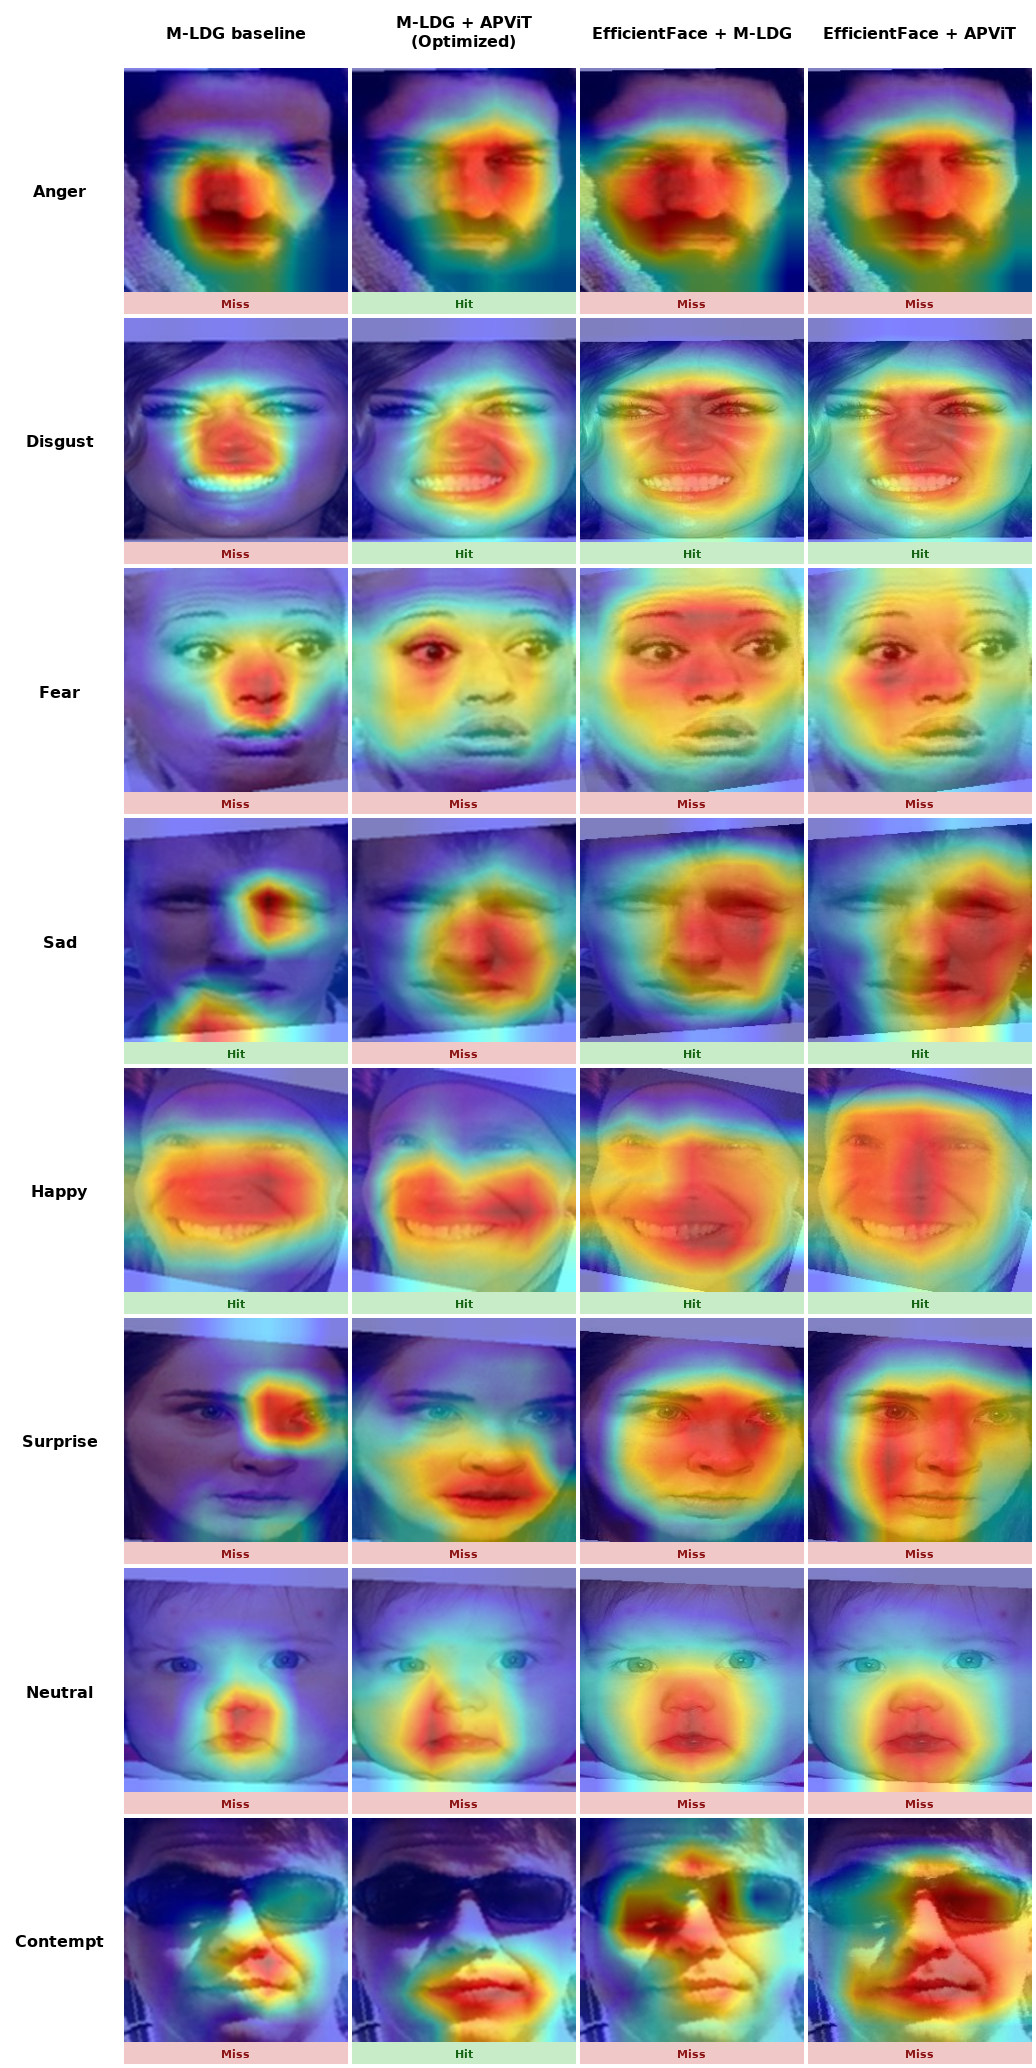
\includegraphics[width=0.65\columnwidth]{../images/chap_results/mixedcamgrid.png}
    \caption[CAM visualizations]{Class activation map (CAM) visualizations for the four of the five main networks used in the cross phase comparison (see table \ref{tab:results-progression}). Each panel shows one validation sample with the model's spatial attention overlaid. Warmer colors indicate higher activation. Hit and miss labels under each image indicate if the sample is correctly or incorrectly classified.}
    \label{fig:results-cam}
\end{figure}

\newpage
